%%%%%%%%%%%%%%%%%%%%%%%%%%%%%%%%%%%%%%%%%%%%%%%%%%%%%%%%%%%%%%%%%%%%%%
% LaTeX Example: Project Report
%
% Source: http://www.howtotex.com
%
% Feel free to distribute this example, but please keep the referral
% to howtotex.com
% Date: March 2011 
% 
%%%%%%%%%%%%%%%%%%%%%%%%%%%%%%%%%%%%%%%%%%%%%%%%%%%%%%%%%%%%%%%%%%%%%%
% How to use writeLaTeX: 
%
% You edit the source code here on the left, and the preview on the
% right shows you the result within a few seconds.
%
% Bookmark this page and share the URL with your co-authors. They can
% edit at the same time!
%
% You can upload figures, bibliographies, custom classes and
% styles using the files menu.
%
% If you're new to LaTeX, the wikibook is a great place to start:
% http://en.wikibooks.org/wiki/LaTeX
%
%%%%%%%%%%%%%%%%%%%%%%%%%%%%%%%%%%%%%%%%%%%%%%%%%%%%%%%%%%%%%%%%%%%%%%
% Edit the title below to update the display in My Documents
%\title{Project Report}
%
%%% Preamble
\documentclass[paper=a4, fontsize=11pt abstract]{scrartcl}
\usepackage[T1]{fontenc}
\usepackage{fourier}

\usepackage[english]{babel}															% English language/hyphenation
\usepackage[protrusion=true,expansion=true]{microtype}	
\usepackage{amsmath,amsfonts,amsthm} % Math packages
\usepackage[pdftex]{graphicx}	
\usepackage{url}
\usepackage[titletoc,title]{appendix}
\usepackage[boxruled ]{algorithm2e}
\usepackage{listings}
\usepackage{bm}
\usepackage{gensymb}
\usepackage{float}
\usepackage{pythonhighlight}

\usepackage{biblatex}
\addbibresource{sample.bib}


%%% Custom sectioning
\usepackage{sectsty}
%\allsectionsfont{\centering \normalfont\scshape}
\allsectionsfont{\normalfont\scshape}


%%% Custom headers/footers (fancyhdr package)
\usepackage{fancyhdr}
\pagestyle{fancyplain}
\fancyhead{}											% No page header
\fancyfoot[L]{}											% Empty 
\fancyfoot[C]{}											% Empty
\fancyfoot[R]{\thepage}									% Pagenumbering
\renewcommand{\headrulewidth}{0pt}			% Remove header underlines
\renewcommand{\footrulewidth}{0pt}				% Remove footer underlines
\setlength{\headheight}{13.6pt}

%%% Equation and float numbering
\numberwithin{equation}{section}		% Equationnumbering: section.eq#
\numberwithin{figure}{section}			% Figurenumbering: section.fig#
\numberwithin{table}{section}				% Tablenumbering: section.tab#


%%% Maketitle metadata
\newcommand{\horrule}[1]{\rule{\linewidth}{#1}} 	% Horizontal rule

\title{
		%\vspace{-1in} 	
		\usefont{OT1}{bch}{b}{n}
		\normalfont \normalsize \textsc{Change this to be the report kind} \\ [25pt]
		\horrule{0.5pt} \\[0.4cm]
		\huge Change This To Report Title \\
		\horrule{2pt} \\[0.5cm]
}
\author{
		\normalfont 								\normalsize
        Robert deCarvalho\\[-3pt]		\normalsize
        \today
}
\date{}



%%% Begin document
\begin{document}
\maketitle


\begin{abstract}
This is abstract content if you want an abstract.
This is abstract content if you want an abstract.
This is abstract content if you want an abstract.
This is abstract content if you want an abstract.
This is abstract content if you want an abstract.
This is abstract content if you want an abstract.
This is abstract content if you want an abstract.
This is abstract content if you want an abstract.
This is abstract content if you want an abstract.
\end{abstract}

\section{First Section}
First section content. First section content. First section content.
This is how you cite\cite{einstein} an article.
This is how you cite\cite{dirac} a book.
This is how you cite\cite{knuth-fa} something in a book.
This is how you cite\cite{knuthwebsite} a link.
First section content. First section content. First section content.
First section content. First section content. First section content.
First section content. First section content. First section content.
First section content. First section content. First section content.
First section content. First section content. First section content.
First section content. First section content. First section content.
First section content. First section content. First section content.

\subsection{Subsection}
subsection content. subsection content. subsection content. 
subsection content. subsection content. subsection content. 
subsection content. subsection content. subsection content. 
subsection content. subsection content. subsection content. 
subsection content. subsection content. subsection content. 
subsection content. subsection content. subsection content. 

\paragraph{}
subsection new paragraph. subsection new paragraph. subsection new paragraph. subsection new paragraph. subsection new paragraph. subsection new paragraph. subsection new paragraph.

List items:
\begin{enumerate}
    \item first thing.
    \item second thing.
\end{enumerate}

\begin{figure}[h!]
    \caption{Put a long figure caption describing your figure here..}
    \label{fig:yourFigureLabel}
    \centering
    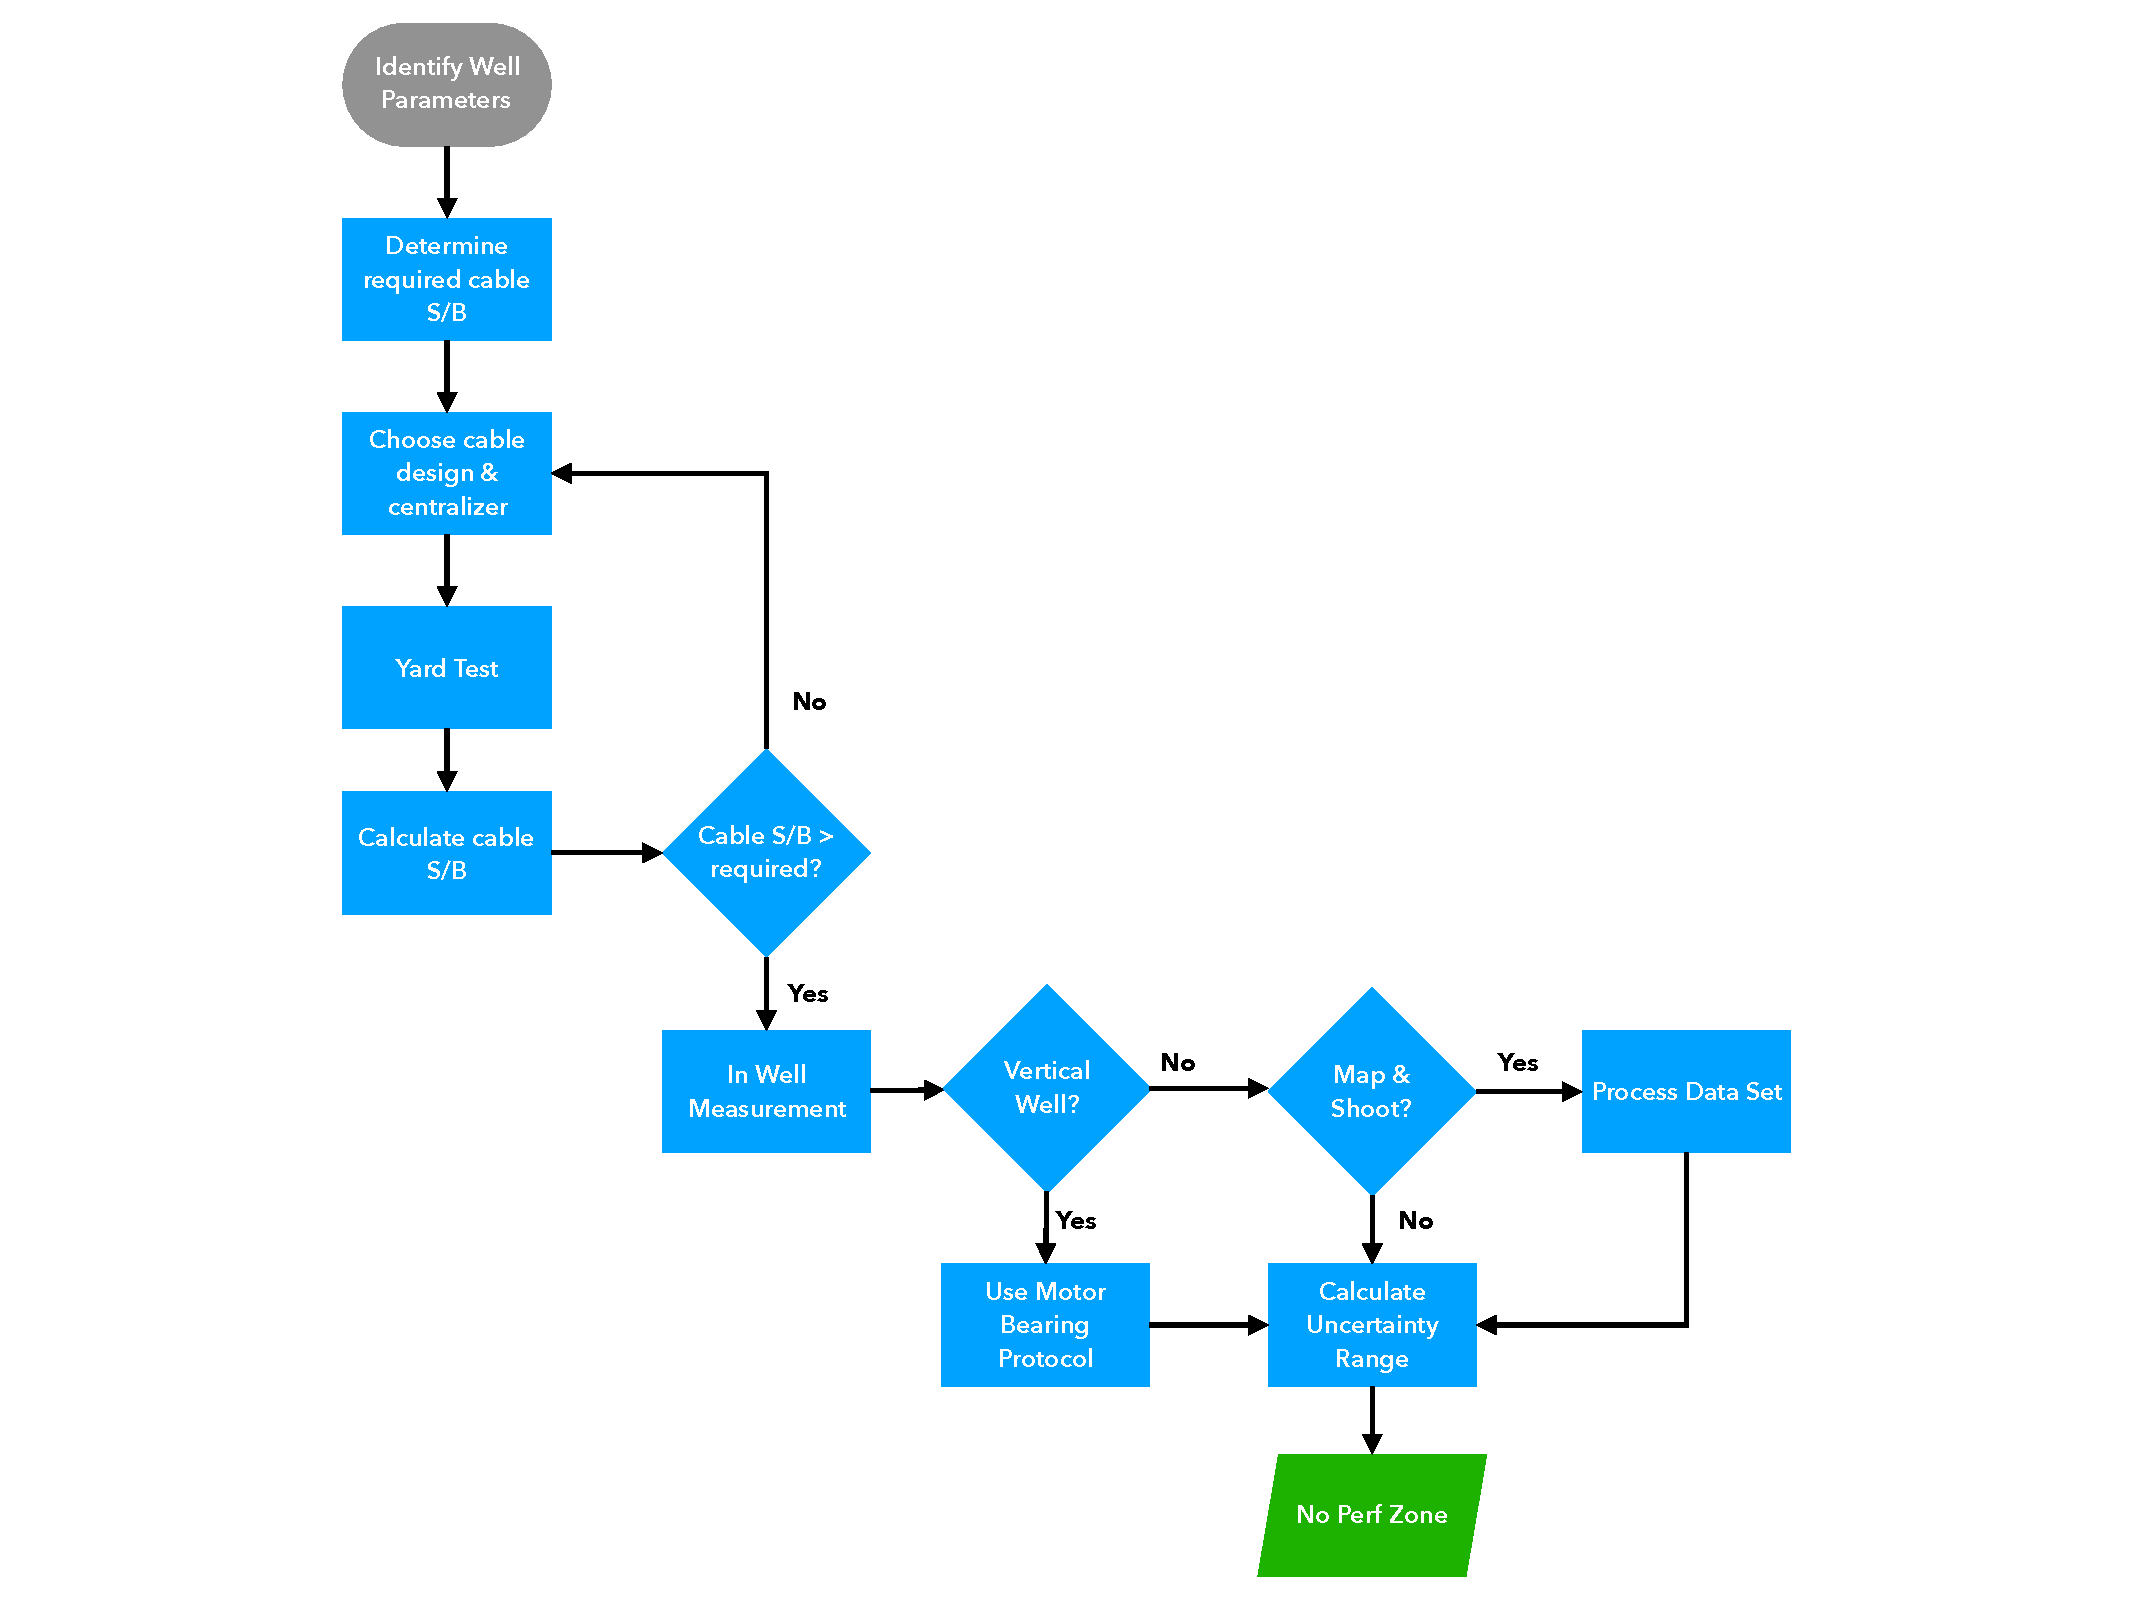
\includegraphics[width=0.5\textwidth]{figures/flow_chart_v2.pdf}
\end{figure}




\section{Equation examples}\label{section:examples}
Here are some example equations.
\begin{equation}
    s = m \cos\left(\phi_s-\phi_m\right) - b\cos\left( \phi_s-\phi_b\right)
\end{equation}

Here is a bunch of text that goes on and on.
Here is a bunch of text that goes on and on.
Here is a bunch of text that goes on and on.
Here is a bunch of text that goes on and on.
Here is a bunch of text that goes on and on.
Here is a bunch of text that goes on and on.
Here is a bunch of text that goes on and on.

\begin{align*}
    s &= \text{cable signal amplitude}\\
    b &= \text{background signal amplitude}\\
    m &= \text{measured signal amplitude}\\
    \phi_s &= \text{cable angle}\\
    \phi_b &= \text{background angle}\\
    \phi_m &= \text{measured angle.}\\
\end{align*}




\pagebreak
\begin{appendices}

\section{Appendix Section}\label{section:first_appendix_section}
Here is a labeled equation
\begin{equation} \label{eq:trig_sig}
    M = s \sin\left(\chi + \phi_s\right) + b \sin\left(\chi + \phi_b\right),
\end{equation}
where
\begin{align*}
        s &= \text{cable signal amplitude} \\
        b &= \text{background signal amplitude.} \\
        \phi_s &= \text{the phase of the cable signal}\\
        \phi_b &= \text{the phase of the background signal}\\
        \chi &= \text{relative bearing as measured by the tool}\\
\end{align*}




\pagebreak
\subsection{This is how you specify algorithms}}
\begin{algorithm}[H] \label{monte_algo}
\SetAlgoLined
\KwResult{Random samples drawn from distribution of bearing correction angles }
 $m \gets$ input the measured signal amplitude\;
 $\mu_s \gets$ input the cable signal mean\;
 $\sigma_s \gets$ input the cable signal standard deviation\;
 $\mu_b \gets$ input the background mean\;
 $\sigma_b \gets$ input the background standard deviation\;
 $N \gets$ input the desired number of samples\;
 $M \gets$ the maximum iterations for finding a triangle solution\;
 $n \gets 0$\;
 $\bm{\theta} \gets$ An array of length $N$\;
 $n \gets 0$\;
 \While{n < N}{
     $i\gets0$\;
     $keepon \gets$ true\;
     \While{$i < M \And  keepon$}{
          $s \gets$ Draw random value from cable signal distribution\;
          $b \gets$ Draw random value from background signal distribution\;
          \uIf{$\left(m-s\right)^2 \leq b ^ 2 \leq \left(m + s\right)^2$}{
              $u \gets$ Draw randomly from $\left[-1, 1\right]$ with equal probability\; 
              $\bm{\theta}\left[n\right] \gets u \cos^{-1}\left(\frac{m^2 + s^2 - b^2}{2ms}\right)$\;
              $n = n + 1$\;
              $keepon\gets$ false\;
          }
          \Else{
              $keepon\gets$ true\;
          }
          $i \gets i + 1$\;
     }
     \If{$i = M$}{
         $\text{Raise an error indicating that no triangle solutions could be found}$\;
     }

 }
 \caption{Bearing correction Monte-Carlo sampling.}
\end{algorithm}

\section{This is how you do python code}
See https://github.com/olivierverdier/python-latex-highlighting
for how to do both inline code like like this \pyth{ser = pd.Series( np.arange(10))}, and code blocks like this

\begin{python}
import pandas as pd
import numpy as np
def get_frame()
    return pd.DataFrame({'a': np.arange(10})
\end{python}

\end{appendices}

\printbibliography

%%% End document
\end{document}